\chapter{Grundlagen}
\section{Distanzmessung mit Ultraschall}
Die Distanzmessung mit Ultraschall ist ein berührungsloses Verfahren. Die Messung erfolgt beruht auf Laufzeitmessung. Der Frequenzbereich von Ultraschalls liegt zwischen 20Khz - 1Ghz (vgl. \cite{ultraschallbereich}) und somit außerhalb des hörbaren Bereichs (20Khz ). \\ Das Frequenzspektrum bei technischen Anwendungen ist kleiner. 
Ein Ultraschallsensor besteht aus einer Sende- und Empfangseinheit. Die Schallwellen werden meist auf Basis des piezoelektrischen Effekts impulsartig ausgesandt und ausgewertet.  Der Ultraschallimpuls pflanzt sich mit Schallgeschwindigkeit im Ausbreitungsmedium fort. Das zu messende Objekt reflektiert die Schallwelle. Die Emfpangseinheit nimmt das entstandene Echo auf. Durch die verstrichene Zeit von der Aussendung bis zum Empfangen des Impulses kann die Entfernung des Objektes bestimmt werden. \\

Dabei gilt:
\begin{align}
d = \frac{1}{2} \cdot t\cdot c\\
\text{mit }  c \approx 340m/s 
\end{align}

Die maximale Messdistanz hängt dabei von der maximal möglichen Intensität der ausgesandter Wellen ab. Die minimale Messdistanz wird durch die Frequenz der Messung bestimmt (vgl. \cite{ultraschallUni}). \\
Prinipbedingt unterliegen Ultraschallsensoren einigen Messfehlern. Dazu gehört, dass schallschluckende Oberflächen eine zu geringe Intensität reflektieren. Dasselbe gilt für Objekte mit rauer Oberfläche. Messfehler können außerdem durch sog. Scheinechos entstehen, wenn der Ultraschallimpuls von mehreren Objekten reflektiert wird. Aufgrund des Öffnungswinkels der Schalwelle ist der gleichzeitige Betrieb mehrerer Sensoren nur	 eingeschränkt möglich. (vgl. \cite{ultraschallBa})

\newpage
\section{Der Schrittmotor}
Der Schrittmotor zählt zu den \acrshort{synchronmaschine}n und besitzt ausgeprägte Statorpolen. Die Motoren werden vor allem in Anwendungen eingesetzt, bei denen hohe Genauigkeit gefordert ist. Anwendungsbeispiele sind Drucker, CD-Laufwerke und computergesteuerte Werkzeugmaschinen. Mit den Motoren können Positionen ohne weitere Regler angesteuerut werden. Schrittmotoren besitzen ein Haltemoment, das ebenfalls in vielen Anwendungen zum Tragen kommt. (vgl. \cite{schrittmotorBa}, S. 2)\\

Prinzipiell folgt bei einem Schrittmotor der Rotor dem sprungförmigen Weiterschalten des Statormagnetfeldes. Dadurch ergibt sich ein schrittweises Drehen um den Schrittwinkel $\alpha$. Nach einer Umschaltung erfolgt die Drehung des Rotors mechanisch bedingt nach einer Verzögerung. Nach einem Einschwingvorgang verharrt der Rotor für einen kurzen Moment in dieser Position.  \autoref{pic:diagrammSchrittmotor} zeigt den zeitlichen Verlauf der mechanischen Winkelgeschwindigkeit  $\Omega$ und des Verdrehwinkels $\beta$ nach dem sprungförmigen Umschalten der Statorwicklung.  

 
\begin{figure}[h]
	\begin{center}
		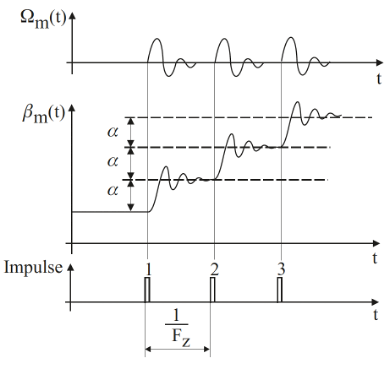
\includegraphics[width=8cm]{DiagrammVerlaufSchrittmotor.png}
		\caption{Zeitlicher Verlauf der mechanischen Winkelgeschwindigkeit und des Verdrehwinkels in Folge elektrischer Impulse in den Statorwicklungen (hier: VR-Schrittmotor); \cite{kleinantriebe} S.433}
		\label{pic:diagrammSchrittmotor}
	\end{center}
\end{figure}


Da der Verdrehwinkel $\beta_M$ ein ganzzahliges Vielfaches des Schrittwinkels $\alpha$ ist, wird eine diskrete Positionierung ohne zusätzliche Sensorik möglich. Diese Art der Positionsbestimmung ist nur möglich, solange das maximale Drehmoment des Schrittmotors nicht überschritten wird. Ist das Lastmoment zu hoch, kommt es zu Schrittervlusten oder gar zum Stillstand.   Für die Ansteuerung eines Schrittmotors wereden durch eine Steuerlogik Impulse erzeugt. Damit wird ein Leistungselektronik-Stellglied gesteuert, das die Statorwicklungen bestromt (vgl. \cite{kleinantriebe}, S. 432). \newline

Auf die folgenden Grundtypen von Schrittmotoren soll nachfolgend näher eingegangen werden:
\begin{itemize}
	\item Reluktanz-Schrittmotor (VR)
	\item Permanenterregert Schrittmotor (PM)
	\item Hybrid-Schrittmotor (HY)
\end{itemize}

\newpage

\subsection{Der \acrshort{reluktanz}-Schrittmotor (VR)}

Beim \acrshort{reluktanz}-Schrittmotor ist der Rotor magnetisch und dessen Zahnteilung ungleich der Polteilung des Stators. Nach einem Umschalten des Statormagnetfeldes bewegt sich der Rotor in die Position des geringsten magnetischen Widerstands (Reluktanz). Diese Stellung wird auch als \acrshort{koinzidenzstellung} bezeichnet. Die Stärke des magnetischen Feldes hängt von der Stromstärke ab. Diese ist veränderlich und verleiht dem Motortyp seine Bezeichnung VR-Motor (\textit{VR = variable reluctance motor}). Kennzeichnend für diesen Motortyp ist das \acrshort{haltemoment} im stromlosen Zustand. 

Für die Anzahl der Schritte je Umdrehung gilt: 

\begin{align}
	z = Z_R\cdot m_S \cdot S \\
	\text{mit } Z_R \text{= Anzahl Rotorzähne und } m_S \text{ = Strangzahl im Stator})
\end{align}

Bei einem \acrshort{vrMotor} mit vier Rotorzähnen und 3 Strängen würde sich somit bei einem Umschaltvorgang ein Verdrehwinkel $\beta$ von 30° einstellen. Für ein größeres Drehmoment werden können bei einem \acrshort{vrMotor} alle Spule gleichzeitig bestromt werden. 

\subsection{Der Permanenterrete Schrittmotor (PM)}
Beim PM-Motor ist der Rotor permanentmagnetisch. Dieser stellt sich ebenfalls in Abhänigigkeit vom Statormagnetfeld in polaritätsrichtige \acrshort{koinzidenzstellung}. Durch den Permanentmagneten bildet der Motor ein Haltemoment im stromlosen Zustand aus. \\ 
Durch die Anzahl $n$ erreger Wicklungen wird der Schrittwinkel $\alpha$ des Rotors bestimmt. Bei Verdopplung von $n$ halbiert sich $\alpha$. Außerdem kann durch $n$ die Betriebsart bestimmt werden. Bleibt $n$ konstant, dreht sich der Rotor im \textit{Vollschrittbetrieb}. Im \textit{Halbschrittbetrieb} wechselt n. In \autoref{pic:halbschrittbetrieb} ist der Verdrehwinkel $\beta_m$ eines PM-Motors im Halbschrittbetrieb dargsetellt. Der Motor besitzt 2 Stränge.  

\begin{figure}[h]
	\begin{center}
		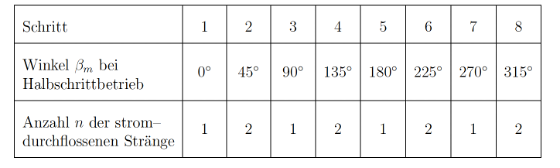
\includegraphics[width=12cm]{halbschrittbetrieb.png}
		\caption{Verdrehwinkel $\beta_m$ bei wechselnder Anzahl erregter Statorwicklungen $n$ (\cite{kleinantriebe} S. 436)}
		\label{pic:halbschrittbetrieb}
	\end{center}
\end{figure}

Der PM-Motor weist ein großes Halte- und Drehmoment auf. Allerdings besitzt der Motortyp eine niedrige Aufllösung. 

\subsection{Der Hybrid-Schrittmotor (HY)}
Der Hybrid-Schrittmotor (HY) vereint die 


\section{MQTT} %Acronym wieder einfuegen!
\acrshort{mqtt} ist ein Protokoll, welches zur digitalen Datenübertragung in ethernet-basierten Systemen dient. Es benötigt nur wenig Bandbreite und Ressourcen und verwendet eine 
Publish/Subscribe - Architektur. Das bedeutet, dass Nachrichten sogenannter Topics von Publishern bereitgestellt und von Subscribern empfangen werden. Der Datenverkehr wird über einen 
zentralen Broker verwaltet. Um die Publish Subscribe Architektur zu verstehen ist es hilfreich die Analogie zum Fernsehen zu bilden. Dabei senjdet ein TV-Sender sein Programm an einen bestimmten Kanal.
Auf diesen Kanal können nun beliebig viele Fernseher (Subscriber) zugreifen. Auch wenn keine aktive Verbindung zwischen Sender und Empfänger aufgebaut wird, erhalten beliebig viele Empfänger die benötigten Daten.
In \autoref{pic:mqttbroker} ist zu erkennen, wie die Daten nicht zwischen Publisher und Subscriber direkt, sondern über den zentralen Broker versendet werden. (Vgl. \cite{mqtt})

\begin{figure}[h]
    \begin{center}
        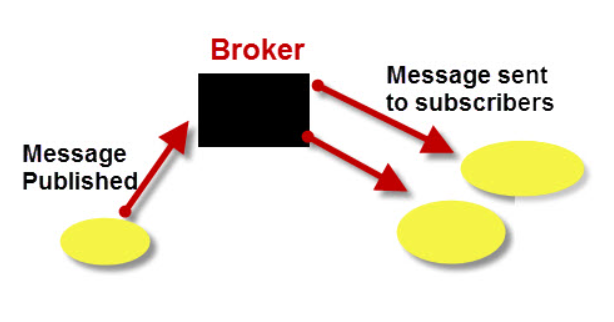
\includegraphics[width=8cm]{mqttbroker.png}
        \caption{\acrshort{mqtt}-Datenübertragung über den Broker}
        \label{pic:mqttbroker}
    \end{center}
\end{figure}